\documentclass{article}

%opening
\title{Simulating Different Receivers in a Rayleigh, SISO Environment\\
\large Winter Intern Seminar (Project \#1)}
\author{노용재\thanks{Intelligent Communication Systems (ICS) Lab.}}
\date{2023-1}

\usepackage{kotex} % korean
\usepackage[margin=1in]{geometry} % 둘레 margin
\usepackage{matlab-prettifier}
\usepackage{amsmath}
\usepackage{graphicx} % image
\usepackage{subcaption} % subfigure

\newcommand{\bd}{\textbf} % bold
\providecommand{\abs}[1]{\lvert#1\rvert}
\graphicspath{{./img/}}

\begin{document}

\maketitle

모든 실험은 다음의 조건하에 진행되었다.

\begin{itemize}
  \item Es/N0는 -2dB~20dB(2dB 간격)
  \item SISO; Single Input, Single Output
\end{itemize}
\section{Binary Moduation}
\bd{공통조건}
\begin{lstlisting}[style=Matlab-editor,
frame=single,
numbers=left,]
NumberIteration = 10^4;
LengthBitSequence = 10^2;

EbN0_dB = -2 : 1 : 20;
EbN0 = db2pow(EbN0_dB);
\end{lstlisting}
\subsection{ZF(Zero-forcing)}
\begin{lstlisting}[style=Matlab-editor,
frame=single,
numbers=left,]
ErrorCount_ZF = zeros(1, length(EbN0_dB));

for iTotal = 1 : NumberIteration
    BitSequence = randi([0 1], 1, LengthBitSequence); % Bit Generation (BitSequence = rand(1, LengthBitSequence) > 0.5;)
    % SymbolSequence = qammod(BitSequence, 2, 'bin'); % 1 and -1    
    SymbolSequence = 2 * BitSequence - 1; % Symbol (s) Generation; consisting of 1 and -1
    NoiseSequence = (randn(1, length(SymbolSequence)) + 1j * randn(1, length(SymbolSequence))) ./ sqrt(2); % Noise (n) Generation
    H = (randn(1, length(SymbolSequence)) + 1j * randn(1, length(SymbolSequence))) ./ sqrt(2); % Channel (h) Generation
    for indx_EbN0 = 1 : length(EbN0)
        ReceivedSymbolSequence_H = H .* SymbolSequence + NoiseSequence * sqrt(1 / EbN0(indx_EbN0)); % Received Signal (y = hs + n) Generation
        
        % ZF Receiver
        DetectionSymbolSequence_ZF = ReceivedSymbolSequence_H ./ H; % Detection (Zero-Forcing: y / h)
        
        % MMSE Receiver
        rho = EbN0(indx_EbN0);
        w_mmse = conj(H) ./ (H.*conj(H)+1/rho);
        DetectionSymbolSequence_MMSE = ReceivedSymbolSequence_H .* w_mmse;
        
        % MLD Receiver
        arg = ([1 1]' * ReceivedSymbolSequence_H) - ([-1 1]' * H);
        arg = arg .* conj(arg);
        DetectionSymbolSequence_MLD = (arg(1, :)-arg(2, :)) > 0; % TODO: could possibly simplify it more
        
        % Symbol Sequence -> Bit Sequence
        DetectionBitSequence_ZF = real(DetectionSymbolSequence_ZF)>0;
        DetectionBitSequence_MMSE = real(DetectionSymbolSequence_MMSE)>0; % not sure if this is right
        DetectionBitSequence_MLD = DetectionSymbolSequence_MLD;
        
        ErrorCount_ZF(1, indx_EbN0) = ErrorCount_ZF(1, indx_EbN0) + biterr(DetectionBitSequence_ZF, BitSequence);
        ErrorCount_MMSE(1, indx_EbN0) = ErrorCount_MMSE(1, indx_EbN0) + biterr(DetectionBitSequence_MMSE, BitSequence);
        ErrorCount_MLD(1, indx_EbN0) = ErrorCount_MLD(1, indx_EbN0) + biterr(DetectionBitSequence_MLD, BitSequence);
    end
end

scatterplot(SymbolSequence)

BER_Simulation_ZF = ErrorCount_ZF / (LengthBitSequence * NumberIteration);
BER_Simulation_MMSE = ErrorCount_MMSE / (LengthBitSequence * NumberIteration);
BER_Simulation_MLD = ErrorCount_MLD / (LengthBitSequence * NumberIteration);

BER_Theory2_H = berfading(EbN0_dB, 'psk', 2, 1);

% Plot
figure()
semilogy(EbN0_dB, BER_Theory2_H, 'k--');
hold on
%hold on don't know what it does
semilogy(EbN0_dB, BER_Simulation_ZF, 'bo');
semilogy(EbN0_dB, BER_Simulation_MMSE, 'rx');
semilogy(EbN0_dB, BER_Simulation_MLD, 'g^');
axis([-2 20 10^-5 0.5]) % axis([a b c d]) x-axis from a to b, y-axis from c to d
grid on
legend('Theory', 'ZF', 'MMSE', 'MLD');
xlabel('Eb/No [dB]');
ylabel('BER');
title('BER for Binary Modulation');
\end{lstlisting}
\subsection{ZF(Zero-forcing)}
\subsection{MMSE(Minimum Mean Square Error)}
\subsection{MLD(Maximum Likelihood Detection)}
\section{M-ary QAM}
$M=2^2n$ $(n=1,2,3,...)$의 상황을 가정하였다.
한 가지 생각해볼 만한 사항은 Normalization Factor이다. 이 Normalization Factor를 사용하여 평균 전력이 1W가 되게끔 둘 수 있다.

QAM의 일반적인 Constellation Diagram을 살펴보면 실수 $\sqrt{M}$개, 허수 $\sqrt{M}$개의 point를 갖는 것을 알 수 있다.\\
하나의 지점을 하나의 alphabet이라고하자. $M$개의 alphabet은 다음과 같다.
\begin{equation}
alphabet={\pm(2n-1)\pm j\cdot(2n-1)} \qquad n\in{1,2,...,\sqrt{M}}
\end{equation}
신호의 평균전력은 다음과 같이 일반화 가능하다.
\begin{equation}
\begin{split}
E_s=E[\abs{s}^2]&=\frac{1}{M}\sum_{n=1}^M \abs{s_n}^2\\
&=\frac{1}{M}\sum_{n=1}^M \sum_{m=1}^M \abs{(2m-1)^2+(2n-1)^2}\\
&=\frac{1}{M}\cdot4\sum_{n=1}^\frac{\sqrt{M}}{2}[(2n-1)^2\cdot\sqrt{M}]\\
&=\frac{4}{M}\sum_{n=1}^\frac{\sqrt{M}}{2}[4n^2-4n+1]\\
&=\frac{2}{3}(M-1)
\end{split}
\end{equation}
(2)에서의 결과를 토대로 normalization이 이뤄진 alphabet을 구할 수 있다.
\begin{equation}
normalized\quad alphabet=\Big{[}\pm\frac{2n-1}{\sqrt{\frac{2}{3}(M-1)}}\pm j\cdot\frac{2n-1}{\sqrt{\frac{2}{3}(M-1)}}\Big{]} \qquad n\in\{1,2,...,\sqrt{M}\}
\end{equation}
해당 결과를 토대로 다시 평균 전력을 구한다면 $E_s$가 1W임을 확인할 수 있다.\\
\\
%\textit{참고자료}\\
\bd{참고자료}\\
다음은 16-QAM의 Constellation이다.\\
\begin{figure}[!ht]
	\centering
	\begin{subfigure}{0.5\textwidth}
		\centerline{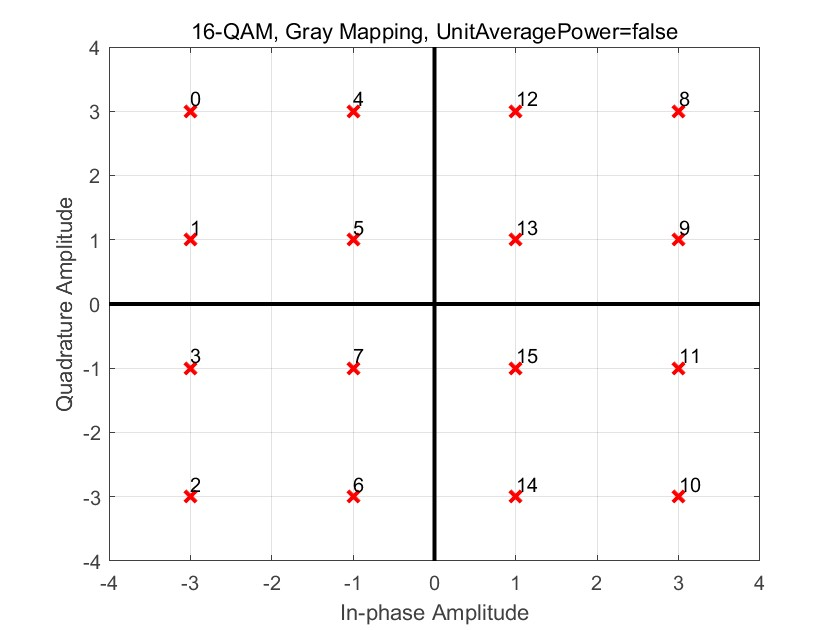
\includegraphics[width=0.8\textwidth]{16qamnonunit.jpg}}
		\caption{Non-normalized Constellation}
	\end{subfigure}%
	\begin{subfigure}{0.5\textwidth}
		\centerline{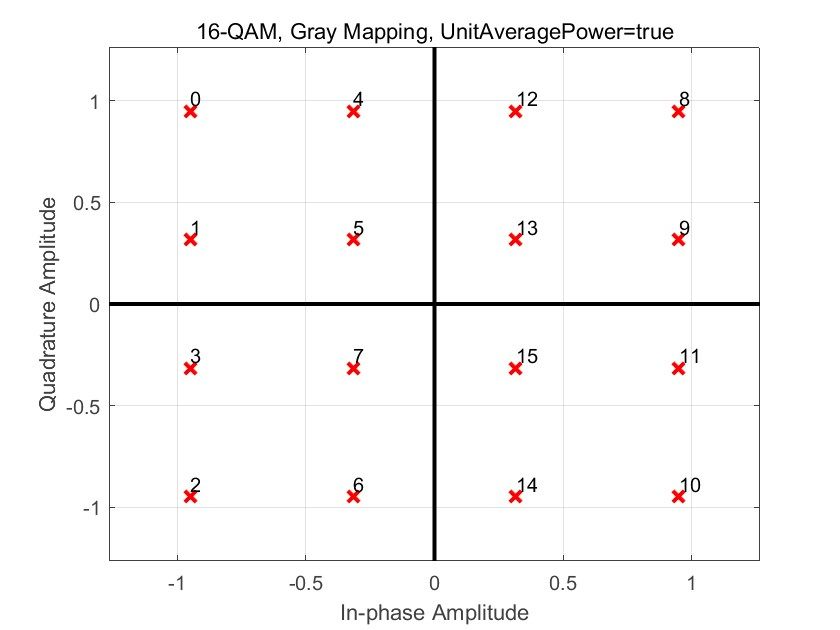
\includegraphics[width=0.8\textwidth]{16qamunit.jpg}}
		\caption{Normalized Constellation}
	\end{subfigure}
	\caption{16-QAM Constellation}
\end{figure}
\\
\subsection{ZF(Zero-forcing)}
\subsection{MMSE(Minimum Mean Square Error)}
\subsection{MLD(Maximum Likelihood Detection)}
\section{과제 외적 의문점}
\begin{itemize}
  \item 왜 $M=4$ 일때의 \textsl{Error Count}는 ZF와 MMSE의 경우 다르지만, $M=16$일 때는 왜 모든 값이 같은가?
\end{itemize}
\end{document}